\subsection{UAP Algorithmus} \label{chap:UAP}
Der hier beschriebene Algorithmus zur Generierung einer \acrfull{uap} basiert auf dem Ansatz von Moosavi-Dezfooli et al. (2017). Ziel ist es, eine Perturbation zu entwickeln, die auf neue Bilder übertragbar ist. Der Algorithmus durchläuft iterativ eine Auswahl von Trainingsbildern und bestimmt jeweils den kürzesten Weg zur Entscheidungsgrenze jedes Bildes. Die dabei erzeugten Perturbationen werden aufsummiert, um eine universelle Perturbation zu erzeugen. Abbildung \ref{fig:uap-paper-figure2} aus Moosavi-Dezfooli et al. \cite{moosavi-dezfooli_universal_2017} illustriert dieses Vorgehen.

\begin{figure}[H]
    \begin{minipage}[b]{0.49\linewidth}
        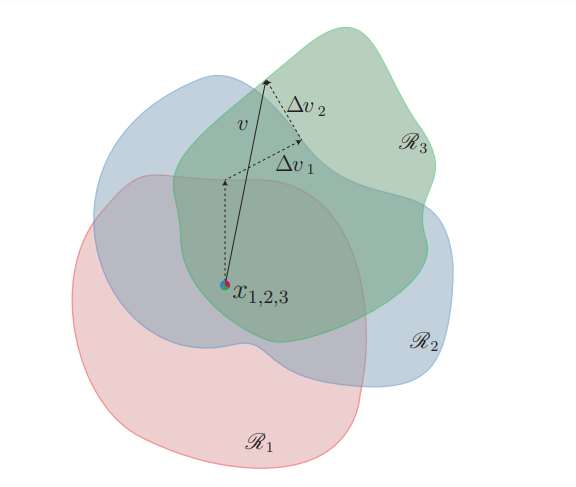
\includegraphics[width=\linewidth]{01-images/04-methodik/UAP-figure2.png}
    \end{minipage}
    \hspace{0.01\linewidth} % Adjust the space between image and caption as needed
    \begin{minipage}[b]{0.49\linewidth}
        \captionof{figure}{``Schematic representation of the proposed algorithm used to compute universal perturbations. In this illustration, data points $x1$, $x2$ and $x3$ are super-imposed, and the classification regions $R_{i}$ (i.e., regions of constant estimated label) are shown in different colors. Our algorithm proceeds by aggregating sequentially the minimal perturbations sending the current perturbed points $x_{i} + v$ outside of the corresponding classification region $R_{i}$'' \cite{moosavi-dezfooli_universal_2017}}
        \label{fig:uap-paper-figure2}
    \end{minipage}
\end{figure}

Bei der Generation der \acrshort{uap}s in dieser Arbeit wird nur eine Teilmenge der positiv gelabelten Trainingsbilder verwendet. Die hier generierten \acrshort{uap}s sind im Gegensatz zum Paper von Moosavi-Dezfooli et al. \cite{moosavi-dezfooli_universal_2017} speziell darauf ausgelegt, positive Klassenbilder fälschlicherweise als negative zu klassifizieren. 

\newpage
\subsubsection{Loss-Funktion $L_{\text{UAP}}$}
Das Optimierungsproblem des Moosavi-Dezfooli et al. \cite{moosavi-dezfooli_universal_2017} wird in dieser Implementierung durch eine selbst definierte Loss-Funktion gelöst, welche die $L_p$-Norm der Perturbationstensor und die inverse \acrlong{bce} Funktion minimiert. Durch die Minimierung der $L_p$-Norm des Perturbationstensors wird sichergestellt, dass die erzeugte Perturbation minimal und somit weniger auffällig ist. Gleichzeitig sorgt die Minimierung der Inverse \acrlong{bce} dafür, dass die aktuelle Perturbation die Klassifikation des Bildes an die Entscheidungsgrenze bringt. Diese Kombination von Loss-Termen stellt sicher, dass die Perturbationen das attackierte Modell täuschen, aber so klein wie möglich sind.

Die Loss-Funktion optimiert $\Delta v$ und sieht wie folgt aus:
\begin{equation}
    L_{\text{UAP}} = \frac{1}{L_{\text{BCE,UAP}}(\hat{y}_i, \hat{y}_{i,\text{adv}}) + \epsilon} + \lambda_{norm} \cdot ||v + \Delta v||_p 
\label{Loss}
\end{equation}

Die verwendete \acrlong{bce} wird wie folgt definiert:
\begin{equation}
L_{\text{BCE,UAP}} = - (\hat{y}_i \cdot \log(\hat{y}_{i,\text{adv}}) + (1-\hat{y}_i) \cdot \log(1-\hat{y}_{i,\text{adv}}))
\label{eq:BCE_UAP}
\end{equation}

\begin{align*}
\lambda_{norm}\text{:} &\text{ Regularisierungsparameter der Matrizennorm.} \\
v\text{:} &\text{ universelle adversarial Perturbation.} \\
\Delta v\text{:} &\text{ Änderung der Perturbation } v \text{.} \\
||\cdot||_p\text{:} & \text{ $L_p$-Norm der Perturbation.} \\
\hat{y}_i\text{:} &\text{ Vorhersage des Modells für das Originalbild ($f(x_{i})$).} \\
\hat{y}_{i,\text{adv}}\text{:} &\text{ Vorhersage des Modells für das perturbierte Bild ($f(x_{i,\text{adv}})$).} \\
\epsilon\text{:} &\text{ kleine positive Konstante für numerische Stabilität.}
\end{align*}

Für die Berechnung eines perturbierten Bildes $x_{i,\text{adv}}$ werden die $x_i$, $v$ und $\Delta v$ element-wise zusammenaddiert: 
$$x_{i,\text{adv}} = x_i + v + \Delta v$$

Der Algorithmus \ref{alg:uap-generierung} iteriert durch jedes Bild einzeln und sucht die Entscheidungsgrenze des aktuellen Bildes, was eine Batch-Grösse von 1 erfordert, wodurch kein Mittelwert in der Loss-Funktion berechnet wird.

Für $\epsilon$ wird ein kleiner Wert wie $10^{-6}$ gewählt, der eine Division durch 0 verhindert, wenn $L_{\text{BCE,UAP}}$ null beträgt. Somit wird das Problem bei der Berechnung der ersten Perturbation gelöst, da zu diesem Zeitpunkt ein Nulltensor vorliegt. 

\newpage
\subsubsection{Technische UAP Umsetzung} \label{chap:technische_umsetzung_uap}

\todo{Tensor aufgrund dani feedback hier erwaehenen fuer delta V}

Die technische Umsetzung des Prozesses zur Generierung der \acrshort{uap}s ist im folgenden Pseudocode beschrieben. Dabei wird die Liste $v$ zurückgegeben, welche alle generierten Perturbationen beinhaltet.

\begin{algorithm}[H]
\caption{Algorithmus für die Generierung von \acrlong{uap}}
\begin{algorithmic}[1]
\label{algo:UAP Algorithmus}
\STATE \textbf{initialize} Liste mit Perturbationen $v$
\FOR{Anzahl Perturbationen $i$}
    \STATE \textbf{initialize} Nulltensor $v_i$
    \WHILE{Fooling Rate $\text{FR}(k) < r$}
        \FOR{Bild $x_i$ $\in$ Trainingsdatensatz $X_{\text{train},+,1:n}$}
        \STATE \textbf{initialize} Nulltensor $\Delta v$
        \STATE \textbf{initialize} Integer $j_{\text{tries}} \gets 0$
            \WHILE{$(f(x_i)\geq k) = (f(x_{i,\text{adv}}) \geq k)$ \textbf{and} $j_{\text{tries}} < t$}         
            \STATE Aktualisiere $\Delta v$ mittels $L_{\text{UAP}}$: $$\Delta v \gets \Delta v - lr_{\text{UAP}} (\frac{\partial L_{\text{UAP}}}{\partial \Delta v})$$
            \STATE Inkrementiere $j_{\text{tries}}$: $$j_{\text{tries}} \gets j_{\text{tries}} + 1$$
            \ENDWHILE
            \STATE Addiere die Perturbation $\Delta v$ auf $v_i$: $$v_i \leftarrow v_i + \Delta v$$
        \ENDFOR
    \ENDWHILE
    \STATE Füge $v_i$ zur Liste $v$ hinzu
\ENDFOR
\STATE \textbf{return} Liste mit Perturbationen $v$
\end{algorithmic}
\label{alg:uap-generierung}
\end{algorithm}

\text{Die Hyperparameter und Inputs des beschriebenen Algorithmus \ref{alg:uap-generierung} sind}
\begin{align*}
i\text{:} &\text{ Anzahl zu generierende Perturbationsbilder.} \\
n\text{:} &\text{ Anzahl Trainingsbilder.} \\
t\text{:} &\text{ Anzahl Versuche, eine bildlokale Perturbation zu finden.}\\
X_{\text{train},+,1:n}\text{:} &\text{ gemischte Teilmenge aller positiven gelabelten Trainingsbilder.} \\
r\text{:} &\text{ gewünschte Mindesttäuschungsrate der Perturbation $v_i$ auf } X_{\text{train},+,1:n}.\\
k\text{:} &\text{ Threshold der Entscheidungsgrenze. } k \in \left] 0; 1 \right[. \\
p\text{:} &\text{ Normparameter der $L_p$-Norm, siehe \nameref{Loss}.}\\
\lambda_{norm},\epsilon\text{:} &\text{ siehe \nameref{Loss}.}\\
lr_{\text{UAP}}\text{:} &\text{ Lernrate der Gewichtsaktualisierung von $\Delta v$.}
\end{align*}

Ein Flow Chart zum \Gls{algorithmus} ist bei Abbildung \ref{fig:05-uap_algorithm} im Anhang zu finden. 

\subsubsection{Wahl des Regularisierungsparameters $\lambda_{norm}$} \label{chap:wahl des Regularisierungsparameters}
In Vorversuchen wurde festgestellt, dass jedes Modell standardmässig unterschiedlich robust gegenüber \acrshort{uap}s ist und dass der Matrizennormalisierungsparameter $\lambda_{norm}$ nicht universell gewählt werden kann. Wenn dieser Parameter zu hoch gewählt wird, wird die Perturbationsgenerierung für manche Modelle instabil und die gewünschte Schwelle der Entscheidungsgrenze $k$ kann nicht erreicht werden. Jedoch darf dieser nicht zu klein gewählt werden, da ein kleinerer Wert zu einer geringen Bestrafung grosser Werte in den Perturbationen führt und diese dadurch stärker wahrgenommen werden können. Wegen dieses Tradeoffs wird ein Wert gesucht, welcher so gross wie möglich ist, jedoch noch stabil bleibt.
\\
\\
Um einen Wert für den Parameter $\lambda_{norm}$ zu wählen, können verschiedene Methoden gewählt werden. In dieser Arbeit wurde folgender Ansatz verwendet: Man beginnt mit dem Wert 0.01 und beobachtet das Verhalten des Algorithmus. Wenn dieser Wert stabil erscheint, indem die Entscheidungsgrenze erreicht wurde, erhöht man $\lambda_{norm}$ auf 0.02 und wiederholt das Verfahren. Danach können die Werte 0.05, 0.1, 0.2, 0.5 und schliesslich 1 ausprobiert werden. Wenn ein Wert sich als instabil erweist, indem die Entscheidungsgrenze $k$ nicht erreicht wird, wird der vorherige Wert endgültig festgelegt. Wenn der Wert 1 sich als stabil erweist, wird er gewählt. Für den Fall, dass sich der Wert 0.01 bereits als instabil erweist, können kleinere Schritte wie 0.005, 0.002, 0.001, 0.0005 usw. ausprobiert werden.
\\
\\
In der folgenden Tabelle \ref{tab:Regularisierungsparameters} werden die gewählten Werte erfasst:

\todo{Befüllen}

\begin{table}[h!]
    \centering
    \begin{subfigure}{0.45\linewidth}
        \centering
        \begin{tabular}{l|l}
            \hline
            \textbf{Modell} & \textbf{$\lambda_{norm}$} \\ 
            \hline
            ResNet50 & 0.05 \\
            \hline
            ResNet18 & $>$1 \\
            \hline
            DenseNet169 & 0.2 \\
            \hline
            EfficientNetV2 M & $>$1\\
        \end{tabular}
        \caption{Gewählte Regularisierungsparameters für den MRI Datensatz}
        \label{tab:BrainTumor}
    \end{subfigure}%
    \hspace{0.05\linewidth} % Adjust horizontal space between tables
    \begin{subfigure}{0.45\linewidth}
        \centering
        \begin{tabular}{l|l}
            \hline
            \textbf{Modell} & \textbf{$\lambda_{norm}$} \\ 
            \hline
            ResNet50 & 0.05 \\
            \hline
            ResNet18 & 0.02 \\
            \hline
            DenseNet169 & 0.005 \\
            \hline
            EfficientNetV2 & 0.0002\\
        \end{tabular}
        \caption{Gewählte Regularisierungsparameters für den COVIDx CXR-4 Datensatz}
        \label{tab:COVIDxCXR4}
    \end{subfigure}
    \caption{Beispiele der gewählten Regularisierungsparameters $\lambda_{norm}$}
    \label{tab:Regularisierungsparameters}
\end{table}


Alternativ könnte für die Wahl von $\lambda_{norm}$ einem automatisierten Ansatz verwendet werden, der die Werte granularer durchsucht. Hier wurde gegen einen solchen Ansatz entschieden, da die Programmierung folgendes Algorithmus zeitintensiver wäre als die Werte manuell zu ermitteln.